\documentclass[conference]{IEEEtran}
\usepackage{cite}
\usepackage{amsmath,amssymb,amsfonts,amsthm}
\usepackage{algorithmic}
\usepackage{graphicx}
\usepackage{textcomp}
\usepackage{xcolor}
\usepackage{mdframed}

\newtheoremstyle{boldstyle}% name
  {\topsep}% space above
  {\topsep}% space below
  {\itshape}% body font
  { }% indent
  {\bfseries}% head font (bold!)
  {.}% punctuation after head
  { }% space after head
  {\thmname{#1}\thmnumber{ #2}\thmnote{ (#3)}}% head spec
\theoremstyle{boldstyle}
% \newtheorem{openquestionx}{Open Question}[section]
% \renewcommand{\theopenquestionx}{\thesection.Q\arabic{openquestionx}}
\newtheorem{openquestionx}{Open Question}
\renewcommand{\theopenquestionx}{Q\arabic{openquestionx}}
\newmdenv[
  skipabove=2pt,
  skipbelow=2pt,
  linewidth=1pt,
  linecolor=blue,
  backgroundcolor=blue!5,
  roundcorner=5pt,
  innertopmargin=2pt,
  innerbottommargin=2pt,
  innerleftmargin=3pt,
  innerrightmargin=3pt
]{openboxq}
\newenvironment{openquestion}
  {\begin{openboxq}\begin{openquestionx}}
  {\end{openquestionx}\end{openboxq}}


\def\BibTeX{{\rm B\kern-.05em{\sc i\kern-.025em b}\kern-.08em
    T\kern-.1667em\lower.7ex\hbox{E}\kern-.125emX}}
\begin{document}

\title{SoK: Preconfirmations}

\author{\IEEEauthorblockN{1\textsuperscript{st} Given Name Surname}
\IEEEauthorblockA{\textit{dept. name of organization (of Aff.)} \\
\textit{name of organization (of Aff.)}\\
City, Country \\
email address or ORCID}
\and
\IEEEauthorblockN{2\textsuperscript{nd} Given Name Surname}
\IEEEauthorblockA{\textit{dept. name of organization (of Aff.)} \\
\textit{name of organization (of Aff.)}\\
City, Country \\
email address or ORCID}
\and
\IEEEauthorblockN{3\textsuperscript{rd} Given Name Surname}
\IEEEauthorblockA{\textit{dept. name of organization (of Aff.)} \\
\textit{name of organization (of Aff.)}\\
City, Country \\
email address or ORCID}
}

\maketitle

\begin{abstract}
This document is a model and instructions for \LaTeX.
\end{abstract}

\begin{IEEEkeywords}
component, formatting, style, styling, insert
\end{IEEEkeywords}

\section{Introduction}

Since the early days of blockchains, it has been well known that by design the system can handle only a limited number of transactions (txs) per second. Meanwhile, traditional centralised payment systems can seamlessly cope with thousands of transactions per second in a quick and efficient way. This scalability issue could seriously impede wide adoption and it was a necessity to solve it to improve Web3 user's experience (UX).

Layer 2s were introduced as a solution to blockchain's scalability trilemma. First formalised by Vitalik Buterin, blockchain's scalability trilemma states that no blockchain system can be decentralised, scalable and secure. The main concept of a layer 2 is to offload transaction volume from its underlying layer 1 blockchain and provide increased throughput with lower transaction fees. \textit{Rollups} are a prime example of a layer 2 solution. Rollup transactions are executed on a separate layer 2 blockchain and aggregated or "rolled-up" in batches that are then recorded on layer 1 as single transactions. Thus, rollups achieve scalability by maintaining the security of layer 1.

Moreover, the transition from Proof of Work (PoW) to Proof of Stake (PoS) in 2022 revolutionised Ethereum and opened up new possibilities. Transaction finality became explicit, block-production rate stabilised, and the whole consensus system became more predictable. Miners were replaced by validators, and time, which was perceived as an abstract concept in the PoW era, was now quantised in epochs divided to 32 slots of 12 seconds. In each slot, one of the validators earns the right to act as a \textit{proposer} and build a new block for the chain. The list of upcoming proposers for the current epoch, is called \textit{lookahead} and is known in advance. Layer 2s have their own \textit{L2 proposer} or \textit{L2 sequencer} who is an entity that batches L2 transactions into L2 blocks and then submits them to the L2 smart contract deployed on L1\cite{W:AnatomyofaSlot:Thetumultuous12secondsduringEthereumslots}.

Furthermore, the idea that block builders can extract value and increase their profit by reordering the transactions they include in a block was becoming more and more prominent. Although the idea of Maximum Extractable Value (MEV) was originally cultivated for PoW, PoS's predetermined slot time and proposer lookahead provided fertile ground for it to flourish. Gradually, MEV extraction became very sophisticated and led to Proposer -- Builder Separation (PBS). In a PBS setting, proposers outsource the duty of building blocks to specialised entities called builders. Flashbots' MEV-Boost became the most predominant implementation of PBS and is so popular at the moment that 90\% of Ethereum blocks are created with it.

However, despite layer 2 creation and PoS's transaction finality explicitness, the barrier of 12 second delay for transaction confirmation persisted. Therefore, \textit{preconfirmations} were proposed as a way to provide users with an early guarantee that their transaction will be included or executed on-chain, giving them a sense of "soft finality".

Although the idea of preconfirming transactions is believed to have originated from earlier Bitcoin projects, the stimulus for preconfirmations was an article called "Based Preconfirmations" by Ethereum Foundation's researcher Justin Drake released in 2023~\cite{W:Basedpreconfirmations}. Ever since, various early implementations, interesting theoretical designs, and conflicting opinions have arisen but they remain scattered and unstructured. 

The purpose of this SoK is to conjugate and systematise knowledge around preconfirmations in a single resource and provide a common language. Our goal is to create a comprehensive and objective report that can be used as an entry point for beginners and a reference point for experts in the field. Finally, we conclude this paper with a list of open challenges to encourage future research on preconfirmations.


\section{Related Work}
This research project builds on previous work conducted in an early effort to aggregate and organise preconfirmation knowledge. Most notably, George Spasov published a glossary for terms related to preconfirmations~\cite{W:PreconfirmationsGlossaryRequirements} and Fabric team put together a collection of resources and articles about preconfirmations~\cite{W:AwesomeBasedPreconfirmations}.


\section{Preliminary}
    \subsection{Preconfirmations (Preconfs)}
    A preconfirmation (preconf) is an early commitment by a proposer to a user that a tx / block will be included in or executed on the chain. The main motivation is to provide users with a fast confirmation guarantee and “soft” finality before the actual confirmation on the L1~\cite{W:Preconfirmations:Explained,W:PreconfirmationsGlossaryRequirements}. Potential use cases of preconfs include reducing tx execution risk, hedging against gas volatility and enhancing trading experience~\cite{W:Preconfirmations:TheFulfillment-DeliveryParadigm}.
    
    \subsection{Types of Preconfs based on execution guarantee} 
    Preconfs can be classified according to the strength of the promise or the execution guarantee of the preconfer. Unless the protocol specifies otherwise, it is at preconfer's discretion to choose what type of preconfs to offer.
        
        \subsubsection{Inclusion Preconfs}
        This type of preconf is a weak commitment of the preconfer. Users receiving this preconf are guaranteed that their tx will be included on chain but they have no assurance that the tx will be executed successfully. Inclusion preconfs can be useful for rudimentary txs like simple transfers, oracle writes and rollup batches~\cite{W:PreconfirmationsforVanillaBasedRollups,W:APricingModelforInclusionPreconfirmations}.
        
        \subsubsection{Execution Preconfs}
        This type of preconf is a strong commitment of the preconfer. It is a commitment that the tx will be included in the chain but also end state after the tx is guaranteed. Due to its nature, it can only be provided by current proposers as future proposers cannot guarantee the initial state before the execution of tx\cite{W:AnalyzingBFTProposer-PromisedPreconfirmations}. Execution preconfs can be useful for more elaborate txs such as DEX trades or arbitrage txs~\cite{W:PreconfirmationsforVanillaBasedRollups}.
    
    \subsection{Preconfirmers (Preconfers)}
    A preconfirmer (preconfer) is an entity that provides users with preconfs. It is vital that a preconfer has the ability to forcefully include a tx on the chain for which he has provided a preconf. 
    
        \subsubsection{Proposers as preconfirmers}
    A proposer that acts as a preconfer is a proposer who has opted in to gain the ability to provide preconfs. To be accepted as a preconfer, the proposer needs to have registered, posted collateral, and accepted the slashing conditions, particularly in the decentralized setting, where such requirements are more important. For centralized L2 preconfers, the conditions may not be as strict~\cite{W:SequencerOpt-InDiscoveryandCommunication,W:Preconfirmations:Explained}.
    
        \subsubsection{Gateways/Delegates as preconfirmers}
    A gateway/delegate that acts as a preconfer is an entity to which preconfer rights were delegated. Influenced by the PBS setting, a gateway is a sophisticated entity that specialises in providing the preconfs instead of the proposer. Proposers can delegate preconfer rights to the gateways and outsource sophistication~\cite{W:ThePreconfirmationGatewayUnlockingPreconfirmations:FromUsertoPreconfer, W:Ahead-of-TimeBlockAuctionsToEnableExecutionPreconfirmations,W:DelegationinBolt:OutsourcingSophisticationWhilePreservingDecentralization}.
    
        \subsubsection{Builders as preconfirmers}
    This category of preconfers is different from the previous two because they can only provide probabilistic preconfs. A builder who acts as a preconfer has no guarantee that the block he builds will be included on chain. Therefore, the type of preconfs that a builder provides are conditional and will be included only if builder's block is selected by a proposer~\cite{W:PreconfirmationFairExchange,W:LeaderlessandLeader-BasedPreconfirmations}.
    
    \subsection{Types of Preconfs based on protocol}
        \subsubsection{Based preconfs}
        A based preconf is a preconf either for L1 or a \textit{based rollup}. An L1-sequenced or based rollup is a rollup whose sequencing is driven directly by the underlying layer 1. In other words, the L2 proposers are also L1 validators. The main advantage of based rollups is that they inherit L1 security, liveness and decentralisation~\cite{W:BasedrollupssuperpowersfromL1sequencing,W:Value-CapturingBasedRollupswithBasedPreconfirmations}.

        For both L1 and based rollups, the preconf is provided by an L1 validator acting as a proposer. The proposer can provide preconfs directly or indirectly by collaborating with a gateway or a builder. 
        
        \subsubsection{Non-based preconfs}
        A non-based preconf is a preconf for a \textit{non-based rollup}. For non-based rollups, L2 proposers providing the non-based preconfs do not need to be L1 validators.
    
\section{Becoming a preconfer}
    Since becoming a preconfer has some strong profit incentives but also comes with power that could potentially be abused, it must be ensured that preconfers commit to behaving honestly. Therefore, in order to become a preconfer, an entity needs to meet some eligibility criteria and accept the punishing conditions. 
    
    \subsection{Preconfer registration}
        \subsubsection{Registry}
        A registry is a smart contract with which validators interact to opt in as preconfers. Prospective preconfers can interact with the registry to register and activate themselves based on the activation criteria of the protocol. The registry can also be used to deactivate preconfers or to check their status~\cite{W:SequencerOpt-InDiscoveryandCommunication}. Moreover, the registry can store important information related to punishment mechanisms of dishonest preconfers, such as blacklists or reputation ratings. Lastly, in an attempt to make preconfer yield accessible to solo-stakers with limited resources, \cite{W:CrediblyNeutralPreconfirmationCollateral:ThePreconfirmationRegistry} suggests integrating an additional collateral delegation method that allows the formation of proposer pools and improves capital efficiency for large operators.
        
        On some occasions, the registry is also entrusted to hold the slashable collateral of the preconfers which is used for the direct monetary punishment of dishonest preconfers. However, many protocols rely on external restaking methods, such as the ones provided by EigenLayer, instead of locking up users' collateral in a smart contract. The main difference between local and outsourced collateral management lies in the reusability of the collateral. On the one hand, registry contracts that double as collateral vaults require dedicated collateral. On the other hand, restaking protocols can reuse the same collateral for other purposes.
        
        At the time of writing, each preconf protocol implements and deploys its own stand-alone registry contract. However, a different approach is receiving general support recently, the Universal Registry Contract (URC)~\cite{W:UniversalRegistryContract}. URC's aim is to create a simple open-source universal contract that replaces the need to create individual registries for each protocol or to rely on external contracts such as restaking platforms. URC standardises the preconfer registration and discovery procedure, handles collateral posting in ETH, and encompasses the slashing and enforcement logic.

        \subsubsection{Eligibility criteria}
        Each protocol has the freedom to set its own eligibility criteria for the preconfers. Generally, preconfers must have the ability to permissionlessly enforce the inclusion / execution of a tx that they issued a preconf for. They should also be discoverable by users and have transparent and low-latency communication with them. Additionally, an honest preconfer should provide timely responses to preconf requests. This can be challenging as they have economic incentive to delay responding to preconf requests~\cite{W:PreconfirmationsGlossaryRequirements}.
        
        \subsubsection{Slashable collateral}
        Each preconfer is obliged to post a slashable collateral to be activated. The collateral acts as an economic disincentive that prevents dishonest behaviour. Any malicious preconfer action--intentional or accidental--that violates the slashing conditions leads to slashing of the preconfer’s collateral. The more serious the offense, the harsher the punishment~\cite{W:Preconfirmations:Explained}.
        
    \subsection{Preconfer faults and punishing conditions} \label{Preconfer faults and punishing conditions}
Preconferent faults (see Fig.~\ref{preconfer fault tree}) are offenses that preconfers should avoid committing because if they do not, they will be penalised. The punishing conditions are put in place to ensure that preconfers will behave honestly and honour their preconf promises and avoid preconfer faults. 
    
    Preconfer punishments always economic consequences but they can be direct or indirect. Direct economic punishments involve collateral slashing. Punishing conditions that can lead to slashing are also called slashing conditions. Indirect economic punishments include blacklisting, orderflow loss, and reputation downgrading~\cite{W:PreconfirmationFairExchange}. 
    
    Violating a punishing condition triggers the enforcement mechanism responsible for punishing the dishonest preconfer. Every preconfer must opt into these conditions as specified by the protocol for which they are providing preconfs~\cite{W:Basedpreconfirmations}. Each protocol's has its own enforcement mechanism (EM) smart contract where its protocol-specific punishing conditions are documented. Any protocol that chooses to adapt the aforementioned URC concept, can also inherit its universal punishing conditions.
    
        \subsubsection{Equivocating response}
        This category incorporates faults that occur when a preconfirmed tx is not included onchain at all. The faults of this category can be further classified into two subcategories.
        \paragraph{Liveness fault}
        A liveness fault occurs when the preconfer misses the slot and therefore the preconf tx is not included onchain. \textcolor{red}{Since this can be accidenal and can potentially be caused by non-malicious behaviour, the punishment for the preconfer may be less harsh. However, as such faults may be indistinguishable from malicious behaviour, they may also need to be punished severely~\cite{W:Basedpreconfirmations}EXPLAIN WHEN IT IS ACCIDENTAL AND WHEN NOT}. To prevent accidental liveness slashing, \cite{W:AvoidingAccidentalLivenessFaultsforBasedPreconfs} suggests a chained preconf system where following preconfers can honour a preconf that was not fulfilled by the active preconfer due to liveness failure.
        % Good opportunity to present specific discussions on pros and cons of both types of slashing.  
        \paragraph{Safety fault}
        A safety fault occurs when the preconfer has not missed the slot yet the preconf tx is not included onchain. This is a serious fault that should never happen and the preconfer can even be fully slashed for it. As this fault cannot happen by accident, the punishment is expected to be more severe than the equivalent punishment for liveness faults. Nevertheless, each protocol can determine the severity of each fault and liveness faults can potentially be considered as severe as liveness fault~\cite{W:Basedpreconfirmations}.
        
        \subsubsection{Equivocating request conditions}
        This category incorporates faults that occur when a preconfirmed tx is included on chain but the preconfer does not comply with the parameters set by the user. As explained in paragraph \ref{RequestSubsection}, users can set various parameters about the tx they wish to have preconfirmed. Some of these parameters depend on the protocol. If the preconfirmed tx is included/executed but without following the guidelines set by the user, the preconfer might be liable to punishment~\cite{W:DelegationinBolt:OutsourcingSophisticationWhilePreservingDecentralization}.
        
        \subsubsection{Idleness fault}
        This category of faults is quite different from the others because the preconfer never gave a preconf. This fault occurs when a preconfer receives perfectly valid preconf requests but denies providing preconf services. There is a thin line between rejecting or ignoring a valid yet non-profitable preconf request and neglecting preconfer duties. Therefore, these faults are handled by a subjective enforcement mechanism, such as an overseer.


    \begin{figure*}[htbp]
        \centering
        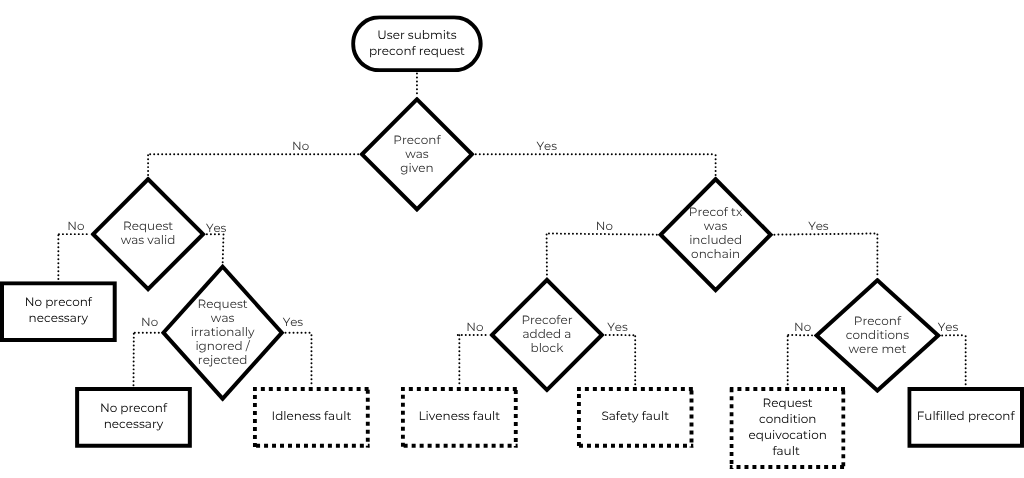
\includegraphics[width=0.9\textwidth]{figures/preconfer fault decision tree.png}
        \caption{Preconfer fault decision tree.}
        \label{preconfer fault tree}
    \end{figure*}
        
        
\section{User -- Preconfer interaction}
    \subsection{Request} \label{RequestSubsection}
    A user who wishes to receive a preconfirmation for a tx submits a signed preconfirmation request to a suitable preconfirmer. The preconf request must include some parameters. There are some parameters that are required by every protocol and some which are protocol-specific. 

    The structure of the proconf request is as follows:

    \begin{itemize}
        \item \textbf{The tx or txs (mandatory for all protocols)} The request must include user's tx so that the preconfer can check its validity before committing to include/execute it.
        Some protocols however allow users to obtain preconf before providing any transaction data~\cite{W:Proposer-CommitmentInfrastructureinEthereum}.
        % In some protocol designs where preconfs are provided by proposers and blocks are built by builders, users can hide their txs from the builders until they get a preconf~\cite{W:PreconfirmationsundertheNOlens}. 
        \item \textbf{Preconfirmation tip (mandatory for all protocols)} The preconf tip is a compensation for the preconf, mutually agreed between user-preconfer. It is atomically binded to the tx so the preconfer cannot redeem the tip without honouring the preconf. The tip is the main incentive for preconfers to provide preconfs and therefore it should be properly priced. 
        
        However, calculating a sufficient tip is non-trivial and can be very challenging. Preconfers are required to solve an online MEV problem and decide whether to accept or reject a preconf request without having a complete image of all the potential txs they can include in the block. This means that the tip should be alluring enough to make the preconfer commit to including/executing a tx instead of rejecting it for the possibility of increasing MEV later within the slot. Subsequently, the preconfer has a motive to delay responding to requests in order to maximise MEV which leads to the fair-exchange problem that will be further investigated in the next paragraphs~\cite{W:StrawmanningBasedPreconfirmations}.
        \item \textbf{Preconf type (depends on the protocol)} Provided that the protocol and/or the preconfer support both inclusion and execution preconfs, users need to specify which type of preconf they want.
        \item \textbf{Deadline (depends on the protocol)} The deadline parameter~\cite{W:PreconfirmationsforVanillaBasedRollups} sets the latest possible L1 slot before which the tx should be honoured. The purpose of this parameter is to hide complexity from the user and improve UX.
        \item \textbf{Bid/Tip decay mechanism (depends on the protocol)} The decay mechanism by Primev~\cite{W:Documentation-BidDecayMechanism} aims to motivate preconfers to provide timely responses to users' requests by gradually reducing the tip until the request finally expires.
        \item \textbf{Preconf penalty (depends on the protocol)} The concept of user defined penalties was first presented by J. Burian~\cite{W:User-DefinedPenalties:EnsuringHonestPreconfBehavior}. According to Burian, instead of relying on a predetermined penalty system, users can define penalty as a parameter. The idea is to allow users and proposers to agree on an appropriate level of crypto-economic security. Similarly, Primev's implementation allows the user to set a slash amount parameter~\cite{W:Documentation-BidStructure}.
        \item \textbf{Latest blockchain state (depends on the protocol)} For execution preconfs, the user needs to specify the state of the blockchain prior to the execution of the tx~\cite{W:AnalyzingBFTProposer-PromisedPreconfirmations}. The user submits the state to ensure that the tx will be executed as expected and the end state after the tx will be guaranteed. A way to do this by including the root state hash in the request.
        \item \textbf{Privacy preferences (depends on the protocol)} Proposed in \cite{W:Towardsanimplementationofbasedpreconfirmationsleveragingrestaking}, setting privacy preferences allows the user to choose which request data will be visible to block proposers and a list of proposers to which the request will be visible. Along the same lines, the user can use the intended preconfer's public key to simplify holding the preconfer accountable in the case of a dishonoured preconf~\cite{W:AnalyzingBFTProposer-PromisedPreconfirmations}.
        \item \textbf{Reverting txs (depends on the protocol)} Primev's implementation allows users to set txs as reverting~\cite{W:Documentation-BidStructure}. A reverting tx can revert without invalidating the request. It is used for txs that are optional or conditional and do not necessarily need to be executed.
    \end{itemize}
    
    
    \subsection{Response}
    After verifying the validity of a preconf request, the preconfer needs to return a signed, slashable promise or a rejection. Generally, preconfers should be incentivised by the protocol to provide timely responses to users in order to improve UX.
    
    A preconf response accepting a request is essentially a preconfirmation (preconf), i.e. a commitment by the preconfer to include/execute a tx. Additionally, rejections do not necessarily constrain preconfer from including the tx in the block unless they are specified by the protocol as non-commitments~\cite{W:SolutionstothePreconfFairExchangeProblem}. Non-commitments are slashable commitments by the preconfers to not include the tx. 

    Similarly to the request, the response has its own parameters. Some of them are always required regardless of the protocol, while others are required by the protocol.

    The structure of the proconf response is as follows:

    \begin{itemize}
        \item \textbf{The preconf request (mandatory for all protocols)} The response should contain the request to which it is directed at~\cite{W:Towardsanimplementationofbasedpreconfirmationsleveragingrestaking}.
        \item \textbf{The block number (mandatory for all protocols)} Preconfer should disclose the number of the block that contains the preconfirmed tx~\cite{W:PreconfirmationsforVanillaBasedRollups}.
        \item \textbf{Preconfer's signature (mandatory for all protocols)} By signing the preconf, the preconfer acknowledges the responsibility of honouring it~\cite{W:Towardsanimplementationofbasedpreconfirmationsleveragingrestaking}. 
        \item \textbf{Updated blockchain state (depends on the protocol)} For execution preconfs, the preconfer may be required to provide the updated blockchain state to prove the correctness of tx execution~\cite{W:AnalyzingBFTProposer-PromisedPreconfirmations}.
    \end{itemize}
    
    
    \subsection{Verification and enforcement of preconfs}
    The final act of the user -- preconfer interaction is the step of verification and enforcement. In this step it needs to be verified that the preconf is fulfilled and the tx is indeed included/executed as specified on the user request. In case the preconfer has violated any of the punishing conditions, the enforcement mechanism will be triggered to punish him. Any accused preconfer who fails to submit evidence against the claim will suffer the consequences~\cite{W:AnalyzingBFTProposer-PromisedPreconfirmations}.

    Although the main idea of an enforcement mechanism is always the same, there are multiple mechanisms with different approaches. The key diffrences between them are whether they are permissionless or permissioned, the type of proof they require to be triggered and the type of enforcement~\cite{W:PreconfirmationFairExchange}.

    In a permissioned setting, punishment through the EM is initiated by a member of the overseer committee. The committee is composed of trusted and whitelisted entities explicitly designated by the protocol. Generally, the proofs required to initiate punishment in this environment are less rigorous.  As long as the committee reaches consensus that a dishonest preconfer should punished, EM can be triggered without further proof. Naturally, this could raise concerns about centralisation, censorship or liveness~\cite{W:PreconfirmationFairExchange}.

    In a permissionless setting, anyone can act as an overseer to initiate punishment via EM on condition that they can prove malicious behaviour. Contrary to a permissioned environment, in this environment, the overseer is required to submit conclusive and indisputable evidence to back up the claim. Furthermore, protocol participants are given economic incentives to act as overseers~\cite{W:GitHub-UniversalRegistryContract,W:GitHub-ExampleSlasherImplementations,W:PreconfirmationFairExchange}. 

    The types of enforcement are closely related to preconfer punishments. As explained in paragraph \ref{Preconfer faults and punishing conditions}, punishments can directly target preconfer's collateral or indirectly target preconfer's profit from preconfs. Punishments can also be divided into real-time or ex-post depending on when they are enforced.
    
    In real-time punishment, preconfer's actions are closely monitored by an overseer and any misbehaviour is immediately detected preventing preconfer from making any profit. As a result, this system requires overseer liveness to operate. 
    
    Ex-post punishments penalise dishonest preconfers retrospectively. Slashing is the most direct and straighforward ex-post punishment. If any of the slashing conditions is violated, the preconfer losses a predetermined amount of their collateral. Moreover, a preconfer can be temporarily blacklisted, i.e. be deprived of their right to provide preconfs or have their stake temporarily frozen. Other than that, the protocol can limit the preconf orderflow of dishonest preconfers or downgrade their reputation to affect future orderflow~\cite{W:PreconfirmationFairExchange,W:User-DefinedPenalties:EnsuringHonestPreconfBehavior}.

    
    \subsection{Fair-Exchange problem in preconfs}
    The fair exchange problem states that during a mutual exchange of items between two parties, it is vital to guarantee that both parties or neither party receive the expected item. No party should have the ability to gain an advantage by misbehaving or quitting the transaction prematurely~\cite{P:Fairexchangewithasemi-trustedthirdparty}.

    In preconf context, users expect to receive preconfirmation for their transaction and preconfers expect to receive compensation for their service. This is achieved by atomically binding the two transactions and broadcasting the preconf commitment to the network to achieve transparency~\cite{W:ThePreconfirmationGatewayUnlockingPreconfirmations:FromUsertoPreconfer}.
    However, for preconfs, time is of the essence. Therefore, solving the fair-exchange problem just by ensuring that the user receives a preconf and the preconfer receives a tip is simply not good enough. For a preconf to be useful to the user, it needs to have been provided in a timely manner.

    Nevertheless, providing preconfs requires solving an online MEV problem. Preconfers are required to commit to reserving block space which could potentially be used for more profitable transactions. Thus, preconfers that receive preconf requests have a clear motive to withhold preconf promises and delay returning them to users. By doing that they can maximise MEV by collecting more potential txs, reordering txs, or inserting new txs~\cite{W:StrawmanningBasedPreconfirmations}.

    Consequently, the fair-exchange problem in preconfs generates the need to incentivise or oblige preconfers to provide and uphold early preconfs following all conditions specified by the users.

    Previous work has proved that it is impossible to solve the fair-exchange problem without an overseer acting as a judge to resolve any disputes~\cite{P:OntheImpossibilityofFairExchangewithoutaTrustedThirdParty} or cryptoeconomic disincentives~\cite{W:Fairexchangewithoutatrustedthirdparty}. It is also harder to solve for one-shot preconfers than it is for repeated game preconfers that care about their reputation~\cite{W:PreconfirmationFairExchange}. 

    L. Oshitani~\cite{W:BasedPreconfirmationswithMulti-roundMEV-Boost} proposed splitting each slot into a fixed number of rounds and performing multiple MEV-boost auctions. Each round creates partial blocks that are combined into a single block at the end of the slot. Among other benefits put forward by that proposal, it is argued that multi-round MEV-boost auctions will simplify tip pricing and mitigate the fair-exchange problem.

    More specifically, it is suggested to equip users with counteractions that they can use against dishonest preconfers. Since preconfers will be required to provide responses within the round instead of the slot, it is easy to stop sending further preconf requests in the next rounds. Also, by specifying separate deadlines for round and slot, preconfers will be forced to provide early responses before the requests expire. Overall, this creates de facto real-time punishment suitable even for one-shot dishonest preconfers.

    Another important piece of research on the fair-exchange problem for preconfs was put forward by C. McMenamin~\cite{W:PreconfirmationFairExchange}. McMenamin proposed a framework for analysing and comparing protocols addressing the fair-exchange problem for preconfs. Furthermore, the proposition evaluates existing L1 and L2 designs and provides guidelines on enforcement mechanisms and overseers. It concludes that it is better for L2 preconf protocols to adopt solutions that intertwine overseers' and protocol's success and employ slashing and blacklisting punishments. For L1s, there is no concrete recommendation, but it is inferred that a formal overseer is most likely required.

    Other potential solutions to the problem include tracking preconfer reputation or sending the request to multiple preconfers in the lookahead and setting a priority rule that decides which preconfer has the right to the tips~\cite{W:SolutionstothePreconfFairExchangeProblem}. Lastly, \cite{W:ThePreconfirmationGatewayUnlockingPreconfirmations:FromUsertoPreconfer} presents ideas on how gateways could help solving the fair exchange problem by monitoring preconfer behaviour and withholding requests or tips.



\section{Economic viability of preconfs}
    The concept of preconfs is still in an early stage. In order to obtain all-around support, it needs to be ensured that all key participants will have clear economic or practical incentives to adopt it. In this section, we discuss the financial uncertainties and costs of preconfs and delve into research findings and open problems concerning the economic viability of preconfs. 
    
    From a user's perspective, preconfs are a tool that improves user experience by providing faster finality and, potentially, protection from MEV attacks. However, UX improvement has some value on its own, which is very likely to be reflected in the price of transactions. In order to create profit margin for the rest of the key participants and compensate for lost MEV, preconfirmed txs will probably need to be more expensive than regular txs. Thus, preconf viability relies on users being willing to pay a little bit more for this improved UX. 

    From a proposer's perspective things are even more complicated. Proposers are profit-driven, and it should not be expected that they would adopt a protocol as an act of kindness. They would never opt-in to provide preconfs and shoulder further sophistication unless they are given satisfactory economic incentives. The same holds for searchers that will have to adapt to the new system and for gateways that will be designed to have preconf duties delegated to them by proposers. Thus, the viability of preconfs lies in providing earning margins similar to the ones that influenced the transition from the traditional solo block-building to PBS and MEV-boosted blocks.

    These observations raise a series of fundamental and mutually correlated questions that must be addressed if preconfs are to attain widespread adoption~\cite{W:EconomicViabilityofPreconfirmations}. 
    \begin{openquestion} \label{Q_why_proposer}
    Why should a proposer become a preconfer instead of retaining the current MEV-Boost setup?
    \end{openquestion}
    \begin{openquestion} \label{Q_impact}
    {What is the expected impact of preconfs on proposers and searchers' profit and what is the expected difference in revenue, risks and costs compared to the current block-proposing process?}
    \end{openquestion}
    \begin{openquestion} \label{Q_pricing}
    {What are good algorithms and methodologies to price preconfs?}
    \end{openquestion}
    \begin{openquestion} \label{Q_diffs_inc_exec}
    {What are the differences between inclusion and execution preconfs in economic terms?}
    \end{openquestion}
    \begin{openquestion} \label{Q_based_seq_profit}
    Should all revenue from based sequencing be absorbed by L1 proposers or should the rollup itself capture some value?
    \end{openquestion}
    \begin{openquestion} \label{Q_quantify_benefits}
    {Improving UX has multiple direct and indirect benefits for a protocol and all its participants, but how can they be quantified?}
    \end{openquestion}

    Answering question \textbf{\ref{Q_why_proposer}}, the way to motive proposers to become a preconfers is to provide them with economic incentives that will increase their revenue. Since the additional proposer profit will come from users' willingness to pay more for preconfs, there is a trade-off. Preconf tips should be priced so they are expensive enough to encourage proposers to provide preconfs but cheap enough to persuade users that faster finality is worth the extra cost.  

    % Preconfirmations under the NO lens
    An analysis by Chorus One~\cite{W:PreconfirmationsundertheNOlens} addresses question \textbf{\ref{Q_impact}} about the impact of preconfs on proposer and searcher rewards in the current PBS setup. It is projected that proposers could increase their revenues at searchers' expense. On the other hand, searchers will need to adapt their bidding behaviour and employ more sophisticated bidding strategies. With the introduction of preconfs, searchers can no longer rely on private communication with builders who have a probability of winning an auction to build a block. This happens because searchers will be able to receive execution preconf for a transaction directly by the proposer. Therefore, searchers are expected to start biding earlier and more aggressively to have their txs preconfirmed.

    % LEGO 1
    Meanwhile, an analysis by Nethermind \cite{W:EstimatingtheRevenuefromIndependentSub-SlotAuctionPreconfirmations} estimates that proposer's revenue will be significantly reduced with the introduction of independent sub-slot auctions (ISSAs) to facilitate execution preconfs.
        
    ISSAs is a proposal aligned with Multi-round MEV-Boost~\cite{W:BasedPreconfirmationswithMulti-roundMEV-Boost} and suggests splitting slots into rounds of equal length. For each round the proposer holds an independent auction to build sub-blocks which are then combined into a block.

    To perform the impact analysis, the components of proposer's profit were classified into categories. It was then forecasted that for most components the reward decays exponentially as the number of rounds per slot as the number of rounds increases. Overall, it was estimated that 8 rounds can reduce proposer's rewards by 50\% while continuous preconfs (assuming unlimited rounds) can reduce proposer's revenue by 74\% compared to a single round MEV-Boost auction.

    This result emphasises the importance of preconf tips as compensation for proposers. Additionally, it suggests that, in order to be viable, preconfs should be priced to at least match the proposers' loss from providing them. This could also be a first step towards answering question \textbf{\ref{Q_pricing}} about preconf pricing.
    
    % LEGO 2
    Further research by C. McMenamin presents the theoretical concept of dependent sub-slot auctions (DSSAs) for facilitating execution preconfs~\cite{W:AnalysingExpectedProposerRevenuefromPreconfirmations}. According to the analysis, DSSAs can increase proposer's expected revenue compared to MEV-boost even without preconf tips.

    Similarly to ISSAs, there is an auction for every sub-slot the winner of which has the right to build the sub-block of the sub-slot. The main difference between ISSAs and DSSAs is that the auction winner also becomes the \textit{active proposer}. The active proposer is the entity with the right to build the remaining of the Ethereum block, thus entitled to the expected revenue of the rest of the block. The first active proposer of each slot is appointed as defined in the lookahead and is responsible to bundle the sub-blocks together in a block at the end of the slot.

    Overall, the active proposer at any sub-slot has the right to build the sub-block or auction off the position of the active proposer for an amount that is at least as much as the expected revenue for the remainder of the slot. The active proposer can also decide whether to offer preconfs to further increase revenue from preconf tips.

    % LEGO 3
    In contrast to execution preconfs, for inclusion preconfs, proposer's expected profit from offering inclusion preconfs is greater than not offering them~\cite{W:AnalysingExpectedProposerRevenuefromPreconfirmations}. Furthermore, although there is no established pricing method, multiple formal models for pricing inclusion preconfs have been put forward~\cite{W:APricingModelforInclusionPreconfirmations,W:PricingTransactionsforPreconfirmation}.

    As explained in \cite{W:APricingModelforInclusionPreconfirmations}, Block size is limited by the blockchain protocol, yet not all sections of the block-space generate the same revenue for the builder. In fact, txs positioned at the top of the block have much greater value because they are executed first and they can be used for txs that are state-dependent and users are willing to pay more for them. The value of block-space decreases until it reaches its lowest value at the bottom of the block.
    
    Inclusion preconfs only guarantee the inclusion of a transaction which gives the block builder the flexibility to place them anywhere in the block. Therefore, a rational block builder would place txs with inclusion preconfs in the least valuable space of the block to save the more valuable space for txs that can generate more profit. At the same time, a rational user would acquire inclusion preconf for txs that cannot be exploited with MEV extraction.

    The pricing model exploits the idea that inclusion preconfs can be placed in the block-space with the lowest value. It suggests deriving the intrinsic value of inclusion preconfs by calculating the value of that least valuable section of the block. However, it is explained that the actual market price is shaped by many factors such as market supply-demand.

    % Pricing Transactions for Preconfirmation
    A different pricing model was presented by a Chorus One research team~\cite{W:PricingTransactionsforPreconfirmation}. This model agrees that txs should be preconfirmed only if they compensate for inclusion risk and produce expected revenue that is equal or greater than MEV-boost. However, the model follows a slightly alternative approach as it suggests using mid-block txs to price inclusion preconfs. Additionally, instead of explicitly pricing inclusion preconfs, it calculates a threshold expressing priority fee per unit of gas that a tx should have to be preconfirmed.

    Initially, the team categorised txs into three tiers based on their position in the block and demonstrated that, on average, the higher the position, the higher the builder's priority fee per unit of gas. Then, data from tiers 1 and 3 were excluded before training three different models (heuristic-based, linear regression, and random forest) that predict the threshold. Tier 1 data were excluded to reduce bias from private order-flow and MEV txs with high priority fees, tier 3 data were excluded to reduce bias from late tx arrival pricing premium.

    After evaluating the models, it was concluded that the random forest model seems to outperform the other two as it can capture more complex data relationships. Also, the results reveal a clear tradeoff as lower threshold means that more txs are preconfirmed, but the loss from incorrectly priced or unprofitable preconfs is higher.

    Overall, concerning question \textbf{\ref{Q_diffs_inc_exec}} preliminary results of preconf viability research seem to converge to the conclusion that without preconf tips, execution preconfs are generally expected to decrease proposer's expected profit while inclusion preconfs are expected to increase it. Moreover, pricing inclusion preconfs is significantly easier and there is no effective method to price execution preconfs yet.

    % Value-capturing based rollups with based preconfirmations
    For question \textbf{\ref{Q_based_seq_profit}}, current based rollups are designed so that all revenue is captured by the L1 proposer who controls sequencing. \cite{W:Value-CapturingBasedRollupswithBasedPreconfirmations} suggests a new protocol design that enables rollups to capture some value.

    According to the proposal, L1 proposers will be charged for sequencing rights in the form of an auction. Auction's profits will be absorbed by the rollup. Once the lookup of an epoch is known, each proposer of a slot i can bid to gain preconfer rights for a series of consecutive slots ending in slot i. The winner of the auction of each slot inherits the right to interact with rollup's smart contract to propose a new based rollup block. Owning sequencing rights for consecutive blocks can be more profitable than owning rights for two separate blocks which gives incentive to proposers to bid in the auction. Furthermore, L1 sequencers can increase their revenue by providing preconfs.

    As for question \textbf{\ref{Q_quantify_benefits}}, accurately quantifying the benefits and the value of UX improvement remains a challenge. Undoubtedly, enhancing UX improves the protocol and increases user utility and demand. At the same time, preconfs decrease MEV. Computing MEV loss is relatively simple, but calculating the value of increasing utility and demand and estimating a fair price that users would agree to pay for preconfs is still puzzling, especially without relevant data. It is possible that preconf protocols would need to go through a pilot phase of experimentation and data gathering which before they can properly answer this question.

    
\section{Risks \& Considerations} % \section{Additional implications/changes/effects}
    \subsection{ecosystem/everybody/systemic}
    
    centralisation problem % gatways, higher sophistication required means less participants can follow (Delegation in Bolt: Outsourcing Sophistication While Preserving Decentralization, Becoming Based: A Path towards Decentralised Sequencing)

    smart contract risk % trust in the system that is complicated, not battle-tested yet (Credibly Neutral Preconfirmation Collateral: The Preconfirmation Registry, The Preconfirmation Sauna)

    liveness, single point of failure and censorship resistance: depending on the preconf implementation. This is an issue with "streaming" continuous preconfs % slot preconfer has full control (Strawmanning Based Preconfirmations, Based Preconfirmations with Multi-round MEV-Boost)
    
    Latency races: depending on the preconf implementation. This is an issue with "streaming" continuous preconfs % lowest latency to preconfer gives user a priority to preconfs for MEV profit txs (Strawmanning Based Preconfirmations, Based Preconfirmations with Multi-round MEV-Boost)
    
    congestion: depending on the preconf implementation. This is an issue with "streaming" continuous preconfs % spamming with arbitrage attempts (Strawmanning Based Preconfirmations, Based Preconfirmations with Multi-round MEV-Boost)

    \subsection{for preconfers}
    slashing % take on risk, including accidental liveness slashing (Avoiding Accidental Liveness Faults for Based Preconfs)
    
    additional complexity / sophistication requirement % this is linked to slashing, centralisation (Towards an implementation of based preconfirmations leveraging restaking, Analysing Expected Proposer Revenue from Preconfirmations)
    
    Delegation: Slashing can be triggered by delegate action, may involve /enable incorrect attribution of faults  % (Delegation in Bolt: Outsourcing Sophistication While Preserving Decentralization)
    
    legal risk % is it a binding contract, mitigation: discalaimer that they are not legally commited
    
    \subsection{for users}
    
    increased prices % Making preconfs attractive to proposers probably requires increasing gas fees. Also increased demand from improved UX can increase gas prices 
    
    sophisticated user requirement % requesting a preconf entails some additional sophistication, most sophistication could be hidden behind the wallet (Analysing Expected Proposer Revenue from Preconfirmations)
    
    Frontrun hazard for non-preconfirmed txs: preconfs may bring a requirement for everyone to use preconfs, which may be worse UX for some users. Can we have preconfs which are "at least as easy to use as current transactions?" % if everyone is doing preconfs and you don't, you might be in a bad position (Analyzing BFT & Proposer-Promised Preconfirmations)
    
    Deposit requirement: requirement to maintain funds in multiple platforrms, depends on the design (not standard)% some protocols require users to post a collateral (Proposer-Commitment Infrastructure in Ethereum)
    
    \subsection{for Rollups}
    increased delay on transaction execution % not every L1 proposer has opted-in to give preconfs (Analyzing BFT & Proposer-Promised Preconfirmations)
    
    Fallback based preconfer needs to be implemented correctly% Mechanism that ensures liveness by reassigning preconfer rights when there is no active preconfer. This happends when there are no based preconfers left in current epoch or the current preconfers are not responding. (Sequencer Opt-In, Discovery and Communication, Becoming Based: A Path towards Decentralised Sequencing)
    
    trade-off between centralised and decentralised sequencing % centralised: high thoughput, low latency, easy preconfs but it has centralisation, censorship, liveness hazards and trust requirements. Widely adopted based rollups with preconfs can achieve high performance (Becoming Based: A Path towards Decentralised Sequencing)

\section{Implementations \& existing protocols}

        \subsection{ \textbf{Primev's MEV-commit}}
        % https://docs.primev.xyz/v1.1.0/get-started/welcome-to-primev
        % https://docs.primev.xyz/v1.1.0/concepts/rewards-and-slashing/rewards-and-slashing
        % https://ethresear.ch/t/preconfirmation-fair-exchange/21891
        

        \subsection{ \textbf{Chainbound's Bolt}}
        % https://research.chainbound.io/
        % https://research.chainbound.io/delegation-in-bolt-outsourcing-sophistication-while-preserving-decentralization
        % https://research.lido.fi/t/proposal-onboard-bolt-to-the-lido-alliance/7724/2
        % https://research.chainbound.io/examining-the-based-sequencing-spectrum
        % https://research.chainbound.io/exploring-verifiable-continuous-sequencing-with-delay-functions
        
        \subsection{ \textbf{Taiko with Nethermind's enforcement mechanism}}
        % https://taiko.mirror.xyz/ejciROGOGM9L_DuuqM3KloZan0EQR73fJt8qzTZmVzg
        % https://4pillars.io/en/articles/preconfirmation-feat-taiko
        % https://en.theblockbeats.news/news/55848
        % https://taiko.mirror.xyz/7_FNvOGfu81imp6A6EucFDoRcKU6E94j4izNEPiugmE
        % https://ethresear.ch/t/rollup-centric-considerations-of-based-preconfimations/20160
        
        \subsection{ \textbf{Espresso}}
        % https://docs.espressosys.com/network/learn/the-espresso-network
        % https://ethresear.ch/t/preconfirmation-fair-exchange/21891
        
        \subsection{ \textbf{Eth gas}}
        % https://www.ethgas.com/
        % https://docs.ethgas.com/overview
        % https://research.lido.fi/t/introducing-ethgas-and-realtime-proposer-commitments-to-the-lido-community/9018
        % % Collateral: either on their L1 collateral contract or Eigenlayer AVS
        
        \subsection{ \textbf{Luban}}
        % https://luban-1.gitbook.io/tai-yi-v0/mfrlyXSvVliigkr4PsmM/taiyi-overview
        % https://lu-ban.notion.site/Consensus-Based-Preconfirmation-with-Multiple-Concurrent-Proposers-aea7f6a7c138401d83eaef429797b540
        
        \subsection{ \textbf{Rise}}
        % https://docs.risechain.com/rise-stack/based-rollups.html
        
        \subsection{ \textbf{Cairo}}
        % https://github.com/cairoeth/preconfirmations
        % https://ethresear.ch/t/towards-an-implementation-of-based-preconfirmations-leveraging-restaking/19211
        
        % \item \textbf{URC's enforcement mechanism}
        % https://eth-fabric.github.io/website/development/l1-components/urc
        % https://github.com/eth-fabric/urc
        % https://github.com/eth-fabric/urc/blob/main/docs/overview.md
        % https://github.com/eth-fabric/urc/tree/main/example
        % https://enshrined-punch-a86.notion.site/Universal-Registry-Contract-143f46539a18809095adf4a14a5ff216
        
        % \item \textbf{Commit-Boost}
        % https://commit-boost.github.io/commit-boost-client/
        % https://github.com/Commit-Boost
        % https://ethresear.ch/t/based-proposer-commitments-ethereum-s-marketplace-for-proposer-commitments/19517
        % https://ethresear.ch/t/commit-boost-proposer-platform-to-safely-make-commitments/20107
                

\section{Other theoretical designs}
% blockspace futures
% "Proposer-Commitment Infrastructure in Ethereum"
% "Pricing Future Blockspace: A Data-driven Approach"

\section{Open research challenges} % maybe "additional" 


\section{Conclusion}

\section*{Acknowledgements}





\newpage
\bibliographystyle{IEEEtran}
% \bibliographystyle{unsrtnat}

\bibliography{references}


\end{document}

% TO-DO:
% Risks (list the risks, find references, write the section)
% Signify open questions
%   gateways
%   fair exchange
%   registry contract (restake, etc)
%   punishing conditions
%   performance monitoring for preconfers, gateways
%   enforcement mechanism
% add more figures
%   user-preconfer interaction figure
% gateways (add more info?)


% -1    \part{part}
%  0	\chapter{chapter}
%  1	\section{section}
%  2	\subsection{subsection}
%  3	\subsubsection{subsubsection}
%  4	\paragraph{paragraph}
%  5	\subparagraph{subparagraph}

